\documentclass[UTF8,a4paper,12pt,fontset=fandol]{ctexart}
\usepackage[margin=23mm]{geometry}
\usepackage{amsmath,amssymb,booktabs,tabularx,array,graphicx}
\usepackage{caption,xurl,hyperref,placeins,float,needspace}
\newCJKfontfamily\ReportGlyphFont[Path=fonts/]{CourseworkGlyph-Regular.ttf}
\newcommand{\ReportAnimalPronoun}{{\ReportGlyphFont 牠}}
\hypersetup{hidelinks}
\linespread{1.13}
\setlength{\emergencystretch}{1em}
\setlength{\tabcolsep}{5pt}
\renewcommand{\arraystretch}{1.12}
\newcolumntype{Y}{>{\raggedright\arraybackslash}X}
\ctexset{section={format=\Large\bfseries\centering},subsection={format=\large\bfseries},subsubsection={format=\normalsize\bfseries}}
\captionsetup{font=small,justification=centering,singlelinecheck=false,labelsep=quad}
\raggedbottom
\setlength{\intextsep}{10pt plus 2pt minus 2pt}
\AddToHook{cmd/section/before}{\Needspace{6\baselineskip}}
\AddToHook{cmd/subsection/before}{\Needspace{5\baselineskip}}
\AddToHook{cmd/subsubsection/before}{\Needspace{4\baselineskip}}
\pagestyle{plain}
% 在正式提交前填写。请使用 Overleaf 的 XeLaTeX 编译器。
\newcommand{\StudentName}{待填写姓名}
\newcommand{\StudentID}{待填写学号}
\newcommand{\ReportDate}{\today}

\title{具身智能基础作业三\\[0.4em]\large 从零构建中文 GPT 实验报告}
\author{姓名\quad\StudentName\qquad 学号\quad\StudentID}
\date{\ReportDate}

\begin{document}
\maketitle


\section{重要知识点梳理与学习}
\subsection{Transformer 的基本结构}
Transformer 通过注意力在序列位置之间交换信息，并用前馈网络变换每个位置的表示。原始结构用于序列到序列建模，由编码器和解码器组成\textsuperscript{\cite{transformer}}。以翻译为例，编码器读取完整源句，得到包含上下文信息的表示，解码器根据源句表示和已生成的目标前缀预测下一个目标 token，整体关系见图\ref{fig:transformer}。图中概括主要信息流，各子层配合残差连接与归一化。

\begin{figure}[H]
\centering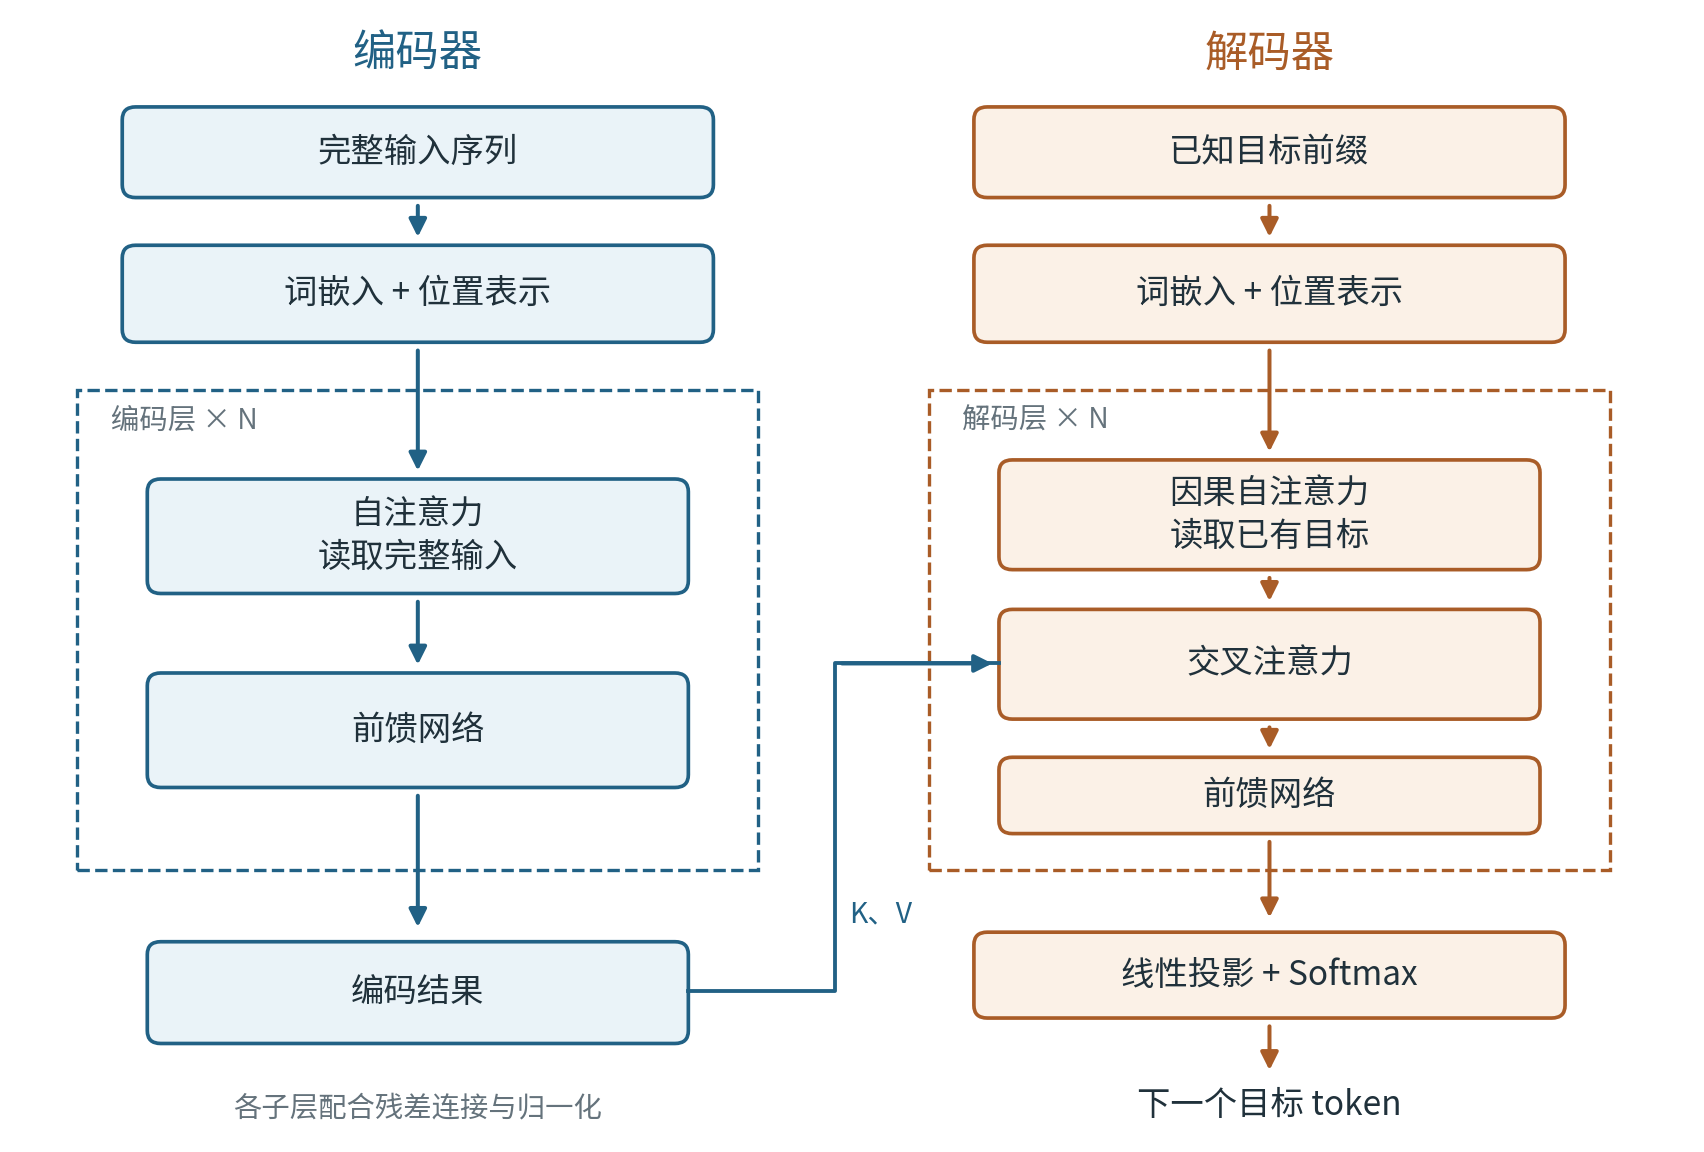
\includegraphics[width=0.91\linewidth]{generated/transformer_overview.png}
\caption{Transformer 结构}\label{fig:transformer}
\end{figure}

编码器的一层包含自注意力和前馈网络。自注意力的查询、键和值均来自本层输入，允许各位置汇总完整源序列中的信息。解码器的一层包含因果自注意力、交叉注意力和前馈网络。因果自注意力只能读取当前目标前缀，交叉注意力则以解码端表示为查询，以编码结果为键和值，将源序列信息引入目标预测。

GPT 采用 decoder-only 结构，把已有文本作为统一前缀，通过因果自注意力向后生成。网络由因果自注意力和前馈子层堆叠而成。新闻标题任务中，新闻、提示和标题前缀共同组成输入序列，后续标题位置通过自注意力读取这些条件。本文实现还采用 Pre-LN、学习式位置嵌入和输入输出权重共享，图\ref{fig:gpt}展示整体信息流与一个 Pre-LN 块，橙色支路表示残差连接。

\subsection{数据准备、分词与输入表示}
文本进入模型前要转为整数序列。数据清洗需要处理 HTML、异常空白、长度和语言比例，再去除重复记录。训练、验证和测试数据分别用于参数学习、配置与检查点选择、最终生成评测。分词器也有需要学习的统计规则，本实验只用训练部分学习词表，以保持数据用途一致。

字节级 BPE 先建立覆盖全部字节的基础字母表，再迭代合并语料中常见的相邻片段，得到固定大小的词表。编码时按已学习的规则将文本转为 token ID，解码时把片段还原为文本。常见中文词语可以成为一个 token，生僻字则可能拆为多个字节片段。词表大小同时影响文本压缩程度、输入嵌入参数量和每次输出的分类规模。

词嵌入矩阵的每一行对应一个 token 的可学习向量。注意力还需要位置信息来区分顺序，本文将词嵌入与学习式绝对位置嵌入相加，得到
\begin{equation}
 H_t^{(0)}=E[x_t]+P[t],\qquad E\in\mathbb{R}^{V\times d},\quad P\in\mathbb{R}^{L\times d}.
\end{equation}
其中 $V$ 为词表大小，$d$ 为隐藏维度，$L$ 为上下文上限。$E[x_t]$ 表示按 ID 查表，$P[t]$ 表示取出第 $t$ 个位置的向量。两组参数随训练共同更新。本文取 $V=16000$、$d=640$、$L=512$，并设置 PAD、BOS 和 EOS 三个特殊 token，分别用于填充、序列起始和文档结束。

\subsection{因果多头自注意力}
设本层输入为 $H$，线性投影得到查询 $Q=HW_Q$、键 $K=HW_K$ 和值 $V=HW_V$，为简化记号省略投影偏置。对于一个注意力头，计算
\begin{equation}
 \operatorname{Attention}(Q,K,V)=\operatorname{softmax}\left(\frac{QK^{\mathsf T}}{\sqrt{d_k}}+M\right)V,
 \quad M_{ij}=\begin{cases}0,&j\le i,\\-\infty,&j>i.\end{cases}
\end{equation}
查询表示当前位置需要匹配的信息，键用于计算各输入位置的匹配得分，值是按权重汇总的内容。每一行的 Softmax 将匹配得分转换为权重，得到各位置值向量的加权和。缩放因子 $\sqrt{d_k}$ 用于控制点积幅度，因果遮罩使当前位置只读取已有 token。多头注意力将隐藏维度划分到不同的头中，分别计算注意力后拼接并投影。

对于 $T$ 个输入 token，注意力分数包含 $T\times T$ 个位置关系。第 $i$ 行只允许第 $1$ 到第 $i$ 列参与 Softmax，因此修改未来 token 不应改变前缀位置的输出。这个性质使训练时所有位置能够并行计算，同时符合逐个预测后续 token 的条件。若当前目标是 $x_{i+1}$，当前位置已经读取 $x_i$，而目标及更后面的 token 受因果遮罩限制。

设注意力头数为 $h$，各头维度为 $d_k=d/h$，多头输出为
\begin{equation}
 \operatorname{MHA}(H)=\operatorname{Concat}(\operatorname{head}_1,\ldots,\operatorname{head}_h)W_O.
\end{equation}
本模型每个头的维度为 $640/10=64$。不同头具有各自的查询、键和值表示，可以对输入中的不同关联分配权重，随后通过输出投影组合各头信息。

\begin{figure}[H]
\centering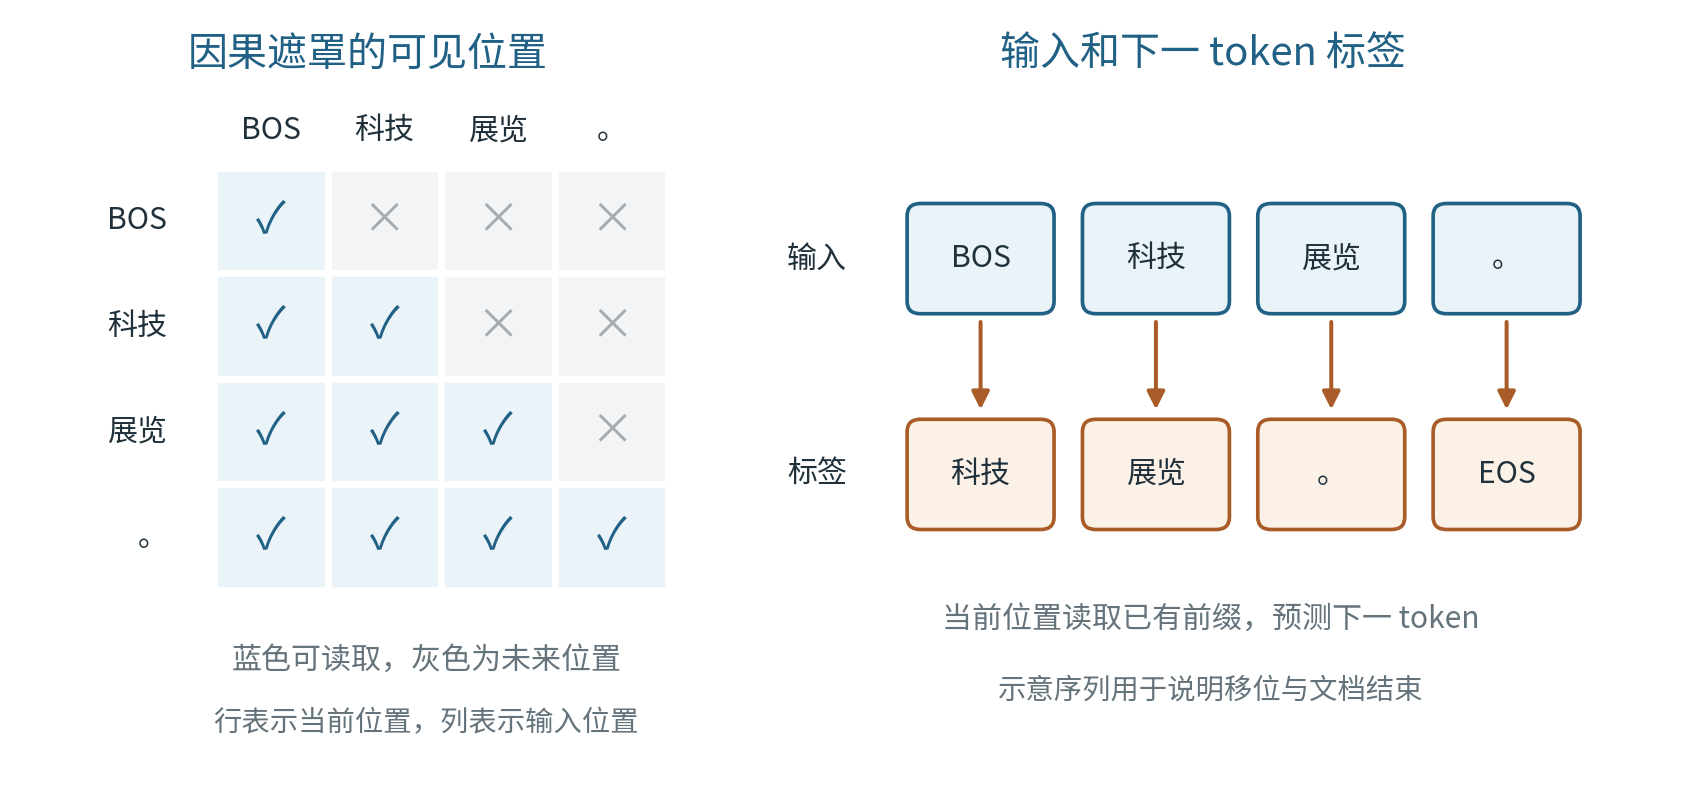
\includegraphics[width=\linewidth]{generated/causal_shift.png}
\caption{因果遮罩与标签移位}\label{fig:causal_shift}
\end{figure}

\subsection{GPT 块、残差连接与输出}
网络采用 Pre-LN 结构，每个 Transformer 块包含注意力和前馈网络两个残差分支
\begin{align}
 U&=H+\operatorname{Dropout}\bigl(\operatorname{MHA}(\operatorname{LN}_1(H))\bigr),\\
 H'&=U+\operatorname{Dropout}\bigl(\operatorname{GELU}(\operatorname{LN}_2(U)W_1+b_1)W_2+b_2\bigr).
\end{align}
其中 MHA 表示注意力聚合与输出投影，注意力概率另施加 dropout。LayerNorm 对单个位置的隐藏维度求均值与方差，再作带可学习缩放和偏移的归一化。前馈网络的中间维度为 $4d$。残差连接保留原有表示，LayerNorm 稳定各层输入尺度。最后经过 LayerNorm 和共享输出矩阵得到 logits，再由 Softmax 给出下一个 token 的概率。

注意力聚合不同位置的信息，前馈网络对每个位置的表示作非线性变换。Pre-LN 在两个分支变换前进行归一化，残差项为信息和梯度提供直接通路。Dropout 在训练时对分支输出作随机置零，验证和推理时关闭。输入嵌入与输出投影共享权重，输出 logits 可写为
\begin{equation}
 z_t=h_tE^{\mathsf T},\qquad
 p_\theta(v\mid x_{\le t})=\frac{\exp(z_{t,v})}{\sum_{u=1}^{V}\exp(z_{t,u})}.
\end{equation}
其中 $h_t$ 为最后一层归一化后的隐藏表示，$v$ 为词表中的候选 token。

\begin{figure}[H]
\centering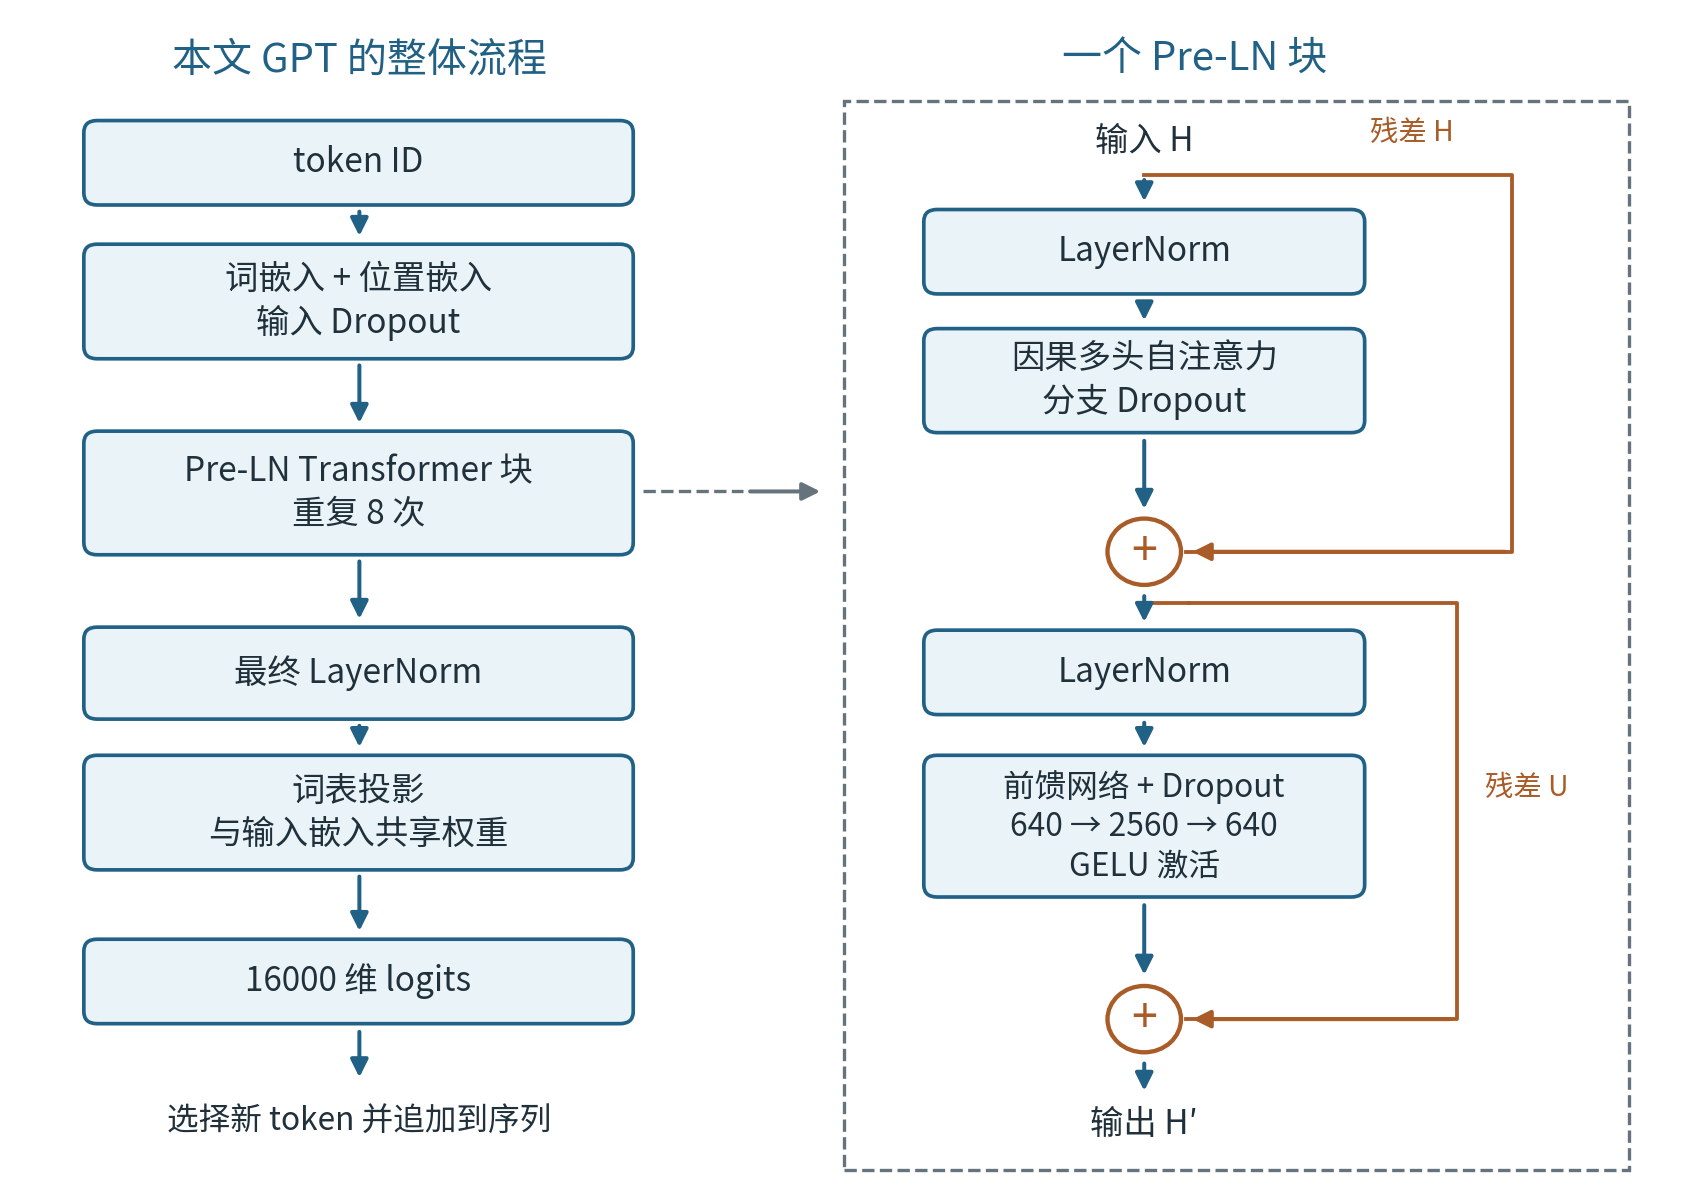
\includegraphics[width=0.94\linewidth]{generated/gpt_preln.png}
\caption{GPT 模型结构}\label{fig:gpt}
\end{figure}

\subsection{自回归目标、预训练与微调}
\subsubsection{下一 token 预测与交叉熵}
GPT 将序列概率分解为各位置的条件概率
\begin{equation}
 p_\theta(x_{1:T})=\prod_{t=1}^{T}p_\theta(x_t\mid x_{<t}).
\end{equation}
其中序列起始位置以 BOS 提供条件。预训练通过大量连续文本学习这一条件分布。

图\ref{fig:causal_shift}左侧表示因果遮罩允许读取的位置，右侧给出输入与标签的移位关系。训练输入与标签相差一个位置。对于 $N$ 个有效目标 token，平均交叉熵为
\begin{equation}
 \mathcal{L}_{\mathrm{PT}}=-\frac{1}{N}\sum_{t=1}^{N}\log p_\theta(x_t\mid x_{<t}).
\end{equation}
因此，最小化交叉熵等价于最大化训练文本的条件对数似然。困惑度定义为
\begin{equation}
 \operatorname{PPL}=\exp(\mathcal{L}_{\mathrm{PT}}).
\end{equation}
在相同分词方式和验证文本下，较低的困惑度表示模型赋予真实后续 token 更高的概率。

设位置 $t$ 的正确标签为 $y_t=x_{t+1}$，该位置的损失为 $\ell_t=-\log p_\theta(y_t\mid x_{\le t})$。结合 Softmax，可得
\begin{equation}
 \frac{\partial\ell_t}{\partial z_{t,v}}=p_\theta(v\mid x_{\le t})-\mathbf{1}(v=y_t).
\end{equation}
正确 token 的概率较低时，其 logit 获得较大的提升方向，其他候选则按预测概率参与调整。梯度经过共享输出矩阵、Transformer 块和输入嵌入反向传播，所有模型参数由同一预测目标联合学习。

\subsubsection{面向标题任务的监督微调}
微调沿用预训练网络，将任务样本组织为“提示、新闻、参考标题、EOS”。模型学习给定新闻与标题前缀后的下一个标题 token，目标为
\begin{equation}
 \mathcal{L}_{\mathrm{SFT}}=-\frac{1}{|\mathcal{S}|}\sum_{t\in\mathcal{S}}\log p_\theta(x_t\mid x_{<t}),
\end{equation}
其中 $\mathcal{S}$ 为标题及 EOS 的目标位置集合。提示与填充位置的目标设为 $-100$，由损失函数忽略。标题位置的损失仍通过网络反向传播，使模型学习如何利用新闻表示。

训练时使用真实标题前缀，逐位置预测后一个标题 token，这一方式称为 teacher forcing。生成时只能使用已经生成的标题前缀，早先的错误可能继续影响后续预测。预训练学习连续文本的广泛下一 token 分布，微调将监督集中于任务输出，因此两阶段损失与困惑度分别在对应目标范围下解释。本文采用全参数微调，所有层均参与更新。

\subsection{参数优化与训练稳定性}
采用 AdamW 更新参数，$\beta_1=0.9$、$\beta_2=0.95$，梯度范数裁剪上限为 1.0。学习率先线性预热，再余弦衰减到峰值的 10\%。使用梯度累积维持有效批量，若第 $j$ 个微批次有 $n_j$ 个监督 token，则累积损失为
\begin{equation}
 \mathcal{L}_{\mathrm{acc}}=\frac{\sum_j\sum_{t\in\mathcal{S}_j}\ell_{j,t}}{\sum_j n_j}.
\end{equation}
各微批次按实际监督 token 数参与平均。

AdamW 根据梯度的一阶矩与二阶矩调整更新尺度。设第 $s$ 步送入优化器的梯度为 $g_s$，则
\begin{align}
 m_s&=\beta_1m_{s-1}+(1-\beta_1)g_s, & v_s&=\beta_2v_{s-1}+(1-\beta_2)g_s^2,\\
 \widehat m_s&=\frac{m_s}{1-\beta_1^s}, & \widehat v_s&=\frac{v_s}{1-\beta_2^s},\\
 \theta_s&=(1-\eta_s\lambda)\theta_{s-1}-\eta_s\frac{\widehat m_s}{\sqrt{\widehat v_s}+\epsilon}, & \epsilon&=10^{-8}.
\end{align}
权重衰减作用于矩阵参数，偏置和归一化参数的 $\lambda$ 为 0。预热使初始更新逐渐增大，余弦衰减使训练后期步长逐渐减小。梯度裁剪在范数超过上限时同比缩放梯度，限制异常批次的更新幅度。

\subsection{自回归生成与任务评价}
训练时，因果遮罩允许完整输入一次前向，所有位置的目标并行计算。推理时每次选出一个新 token，追加到前缀后再进行下一次预测，因此输出长度会直接影响生成时间。

贪心解码选择概率最大的候选。温度采样先将 logits 除以 $\tau>0$，再从分布中抽样，较小的温度使概率更集中。top-k 只保留得分最高的 $k$ 个候选，再归一化抽样。这些设置影响同一模型的生成结果，需要在比较时记录并保持一致。

标题效果使用字符级 ROUGE。保留 Unicode 字母和数字，英文转为小写，再计算字符 n-gram 重合与最长公共子序列。设预测为 $p$，参考为 $r$，$G_n$ 为 n-gram 多重集，则
\begin{align}
 \operatorname{ROUGE}\text{-}n&=\frac{2|G_n(p)\cap G_n(r)|}{|G_n(p)|+|G_n(r)|},\\
 \operatorname{ROUGE}\text{-}L&=\frac{2\operatorname{LCS}(p,r)}{|p|+|r|}.
\end{align}
逐条计算 F1 后取宏平均，表中乘以 100 表示，空输出得零分。

ROUGE-1 反映字符覆盖，ROUGE-2 更重视局部相邻组合，ROUGE-L 还考虑字符顺序。使用字符级指标可以统一中文与英文片段的处理方式。人工标题可能对正文改写或概括，词面重合需要结合内容理解，数字和事件关系则通过生成样例检查。

\FloatBarrier
\section{小参数量 GPT 模型搭建}
\subsection{实现与配置}
采用 PyTorch 基础层实现注意力投影、Transformer 块、模型前向传播和训练循环，架构与训练流程的学习参考 LLMs from Scratch\textsuperscript{\cite{fromscratch}}。模型使用 8 层、10 个注意力头和 640 维隐藏表示，共包含 49,957,120 个独立参数，配置见表\ref{tab:model}。

\begin{table}[H]
\centering\small
\caption{GPT 模型配置}\label{tab:model}
\begin{tabularx}{0.86\linewidth}{Y r}
\toprule 配置项 & 设置 \\ \midrule
Transformer 层数 & 8 \\
注意力头数 & 10 \\
隐藏维度 / 前馈中间维度 & 640 / 2560 \\
上下文长度 & 512 token \\
词表大小 & 16000 \\
Dropout & 0.1 \\
位置表示 & 学习式绝对位置嵌入 \\
输入与输出嵌入 & 权重共享 \\
\bottomrule
\end{tabularx}
\end{table}

词表规模为 $V$、隐藏维度为 $d$ 时，参数量为
\begin{equation}
 Vd+Ld+n_{\mathrm{layer}}(12d^2+13d)+2d=49\,957\,120.
\end{equation}
其中词嵌入包含 10,240,000 个参数，位置嵌入包含 327,680 个参数，8 个 Transformer 块合计 39,388,160 个参数，最终 LayerNorm 包含 1280 个参数。各层的主要张量形状见表\ref{tab:tensors}，$B$ 表示微批量大小，$T\le512$ 表示输入长度。

\begin{table}[H]
\centering\small
\caption{主要张量形状}\label{tab:tensors}
\begin{tabularx}{\linewidth}{Y l}
\toprule 计算阶段 & 张量形状 \\ \midrule
token 与位置嵌入相加 & $(B,T,640)$ \\
查询、键、值的联合线性投影 & $(B,T,1920)$ \\
分头后的 $Q$、$K$、$V$ & 各为 $(B,10,T,64)$ \\
各头注意力分数的逻辑形状 & $(B,10,T,T)$ \\
拼接并投影后的注意力输出 & $(B,T,640)$ \\
前馈网络的中间表示 & $(B,T,2560)$ \\
最终词表 logits & $(B,T,16000)$ \\
\bottomrule
\end{tabularx}
\end{table}

线性层和嵌入矩阵采用均值为 0、标准差为 0.02 的正态初始化，线性偏置初始化为 0。注意力输出投影和前馈网络第二个线性层的标准差再除以 $\sqrt{2n_{\mathrm{layer}}}$，减小多层残差分支初始叠加的幅度。

保留手写注意力和 SDPA 两种实现，正式训练使用 SDPA。测试分别修改序列后半部分，检查前缀 logits 是否保持一致，并比较两种注意力的输出与梯度。另用小型模型拟合可控的下一 token 任务，检查损失能够下降。单元测试还覆盖权重共享、分词往返、标签遮罩和解码约束。

运行环境为 Windows 11、Python 3.12.14、PyTorch 2.6.0+cu124、NumPy 2.2.6 和 Tokenizers 0.21.0，使用 RTX 4060 Laptop 8GB 显卡及 BF16 计算，随机种子取 42。

本次采用 512-token 上下文和微批量 4，预训练与微调分别累积 16 次、8 次梯度，使训练能够在本机单卡完成。

\subsection{本地推理过程}
推理采用评估模式与无梯度前向，先编码提示文本，取最后一个位置的 logits 选择新 token，再把它追加到输入，重复前向传播，直到生成 EOS 或达到长度上限。

续写实验取温度 $\tau=0.8$、top-k 为 40，每次最多生成 64 个新 token。当前实现每步重新计算已有前缀，输入超过窗口时取最近的 512 个 token，生成开销随输入和输出长度增长。

\FloatBarrier
\section{模型预训练}
\subsection{数据准备与训练程序}
数据使用 XL-Sum 简体中文 BBC 新闻\textsuperscript{\cite{xlsum}}，取 text 字段为正文，title 字段为标题。原始训练、验证和测试集分别有 37362、4670 和 4670 篇。进行 HTML 清理、NFKC 规范化和空白合并，保留正文长度 100--10000 字符、中文比例至少 50\%、标题长度 4--80 字符的记录。移除正文开头复制的标题，再依据规范化正文及其前 256 个字符去重。清洗后训练集为 36762 篇，验证集为 4585 篇，测试集为 4662 篇，各记录保留官方分区归属。

清洗过滤了 306 篇记录，跨分区去重移除 387 篇。分词器与模型使用训练集学习，验证集用于检查点选择，测试集用于生成评测。按正文及前缀去重可以处理相同文本，不同措辞的同事件报道仍可能保留。

使用仅在训练集学习的字节级 BPE 词表编码新闻。实际词表将“学校今天举办科技展览。”编码为
\begin{equation}
 [1905,\ 2336,\ 3622,\ 2393,\ 5759,\ 264],
\end{equation}
对应片段依次为“学校”“今天”“举办”“科技”“展览”和“。”，解码后还原原句。这里的汉字、词语与 token 长度并不相同，后续窗口和预算统一按 token 计算。

将训练新闻组织为 BOS、标题、换行、正文和 EOS，拼接后的 token 流长度为 26312816。每次随机抽取 513 个连续 token，构造 512 个输入与下一 token 标签。采样允许窗口跨越文档边界，EOS 标识文档结束。

输入 ID 经过词嵌入查表，与位置 $0$ 到 $511$ 的可学习向量相加，再送入模型。词嵌入与位置嵌入均从随机参数开始训练，随下一 token 目标共同更新。

对于窗口 $x_{1:513}$，实际输入为 $x_{1:512}$，标签为 $x_{2:513}$。前向传播得到 $(B,512,16000)$ 的 logits，计算全部下一 token 标签的交叉熵，按有效目标数归一化后反向传播。完成 16 个微批次的梯度累积后，执行裁剪和一次 AdamW 更新。

预训练执行 3000 个优化器步，微批量为 4，累积 16 次，有效批量为 64。最大学习率设为 $3\times10^{-4}$，预热 100 步，权重衰减为 0.1。每 100 步在固定的 20 个验证批次上估计损失，保存验证损失最低的检查点。验证时关闭 dropout，每次统计 40960 个目标 token。

预训练累计处理 $3000\times64\times512=98\,304\,000$ 个 token，约为训练流长度的 3.74 倍。窗口有放回采样，每次验证使用固定窗口。

\subsection{结果与分析}
预训练固定验证交叉熵由9.7996降至4.7993，困惑度由18026.74降至121.43。最佳检查点位于第3000步，累计处理98,304,000个输入token，训练迭代用时35.5分钟。图\ref{fig:pretrain}显示，损失在前期下降较快，后期下降幅度减小。

\begin{table}[H]
\centering\small
\caption{预训练验证结果}\label{tab:pretrain_checkpoints}
\begin{tabularx}{\linewidth}{Y r r}
\toprule 训练步数 & 平均交叉熵 & 困惑度 \\ \midrule
0 & 9.7996 & 18026.74 \\
1000 & 5.5376 & 254.07 \\
2000 & 4.9623 & 142.92 \\
3000 & 4.7993 & 121.43 \\
\bottomrule
\end{tabularx}
\end{table}

\begin{figure}[H]

\centering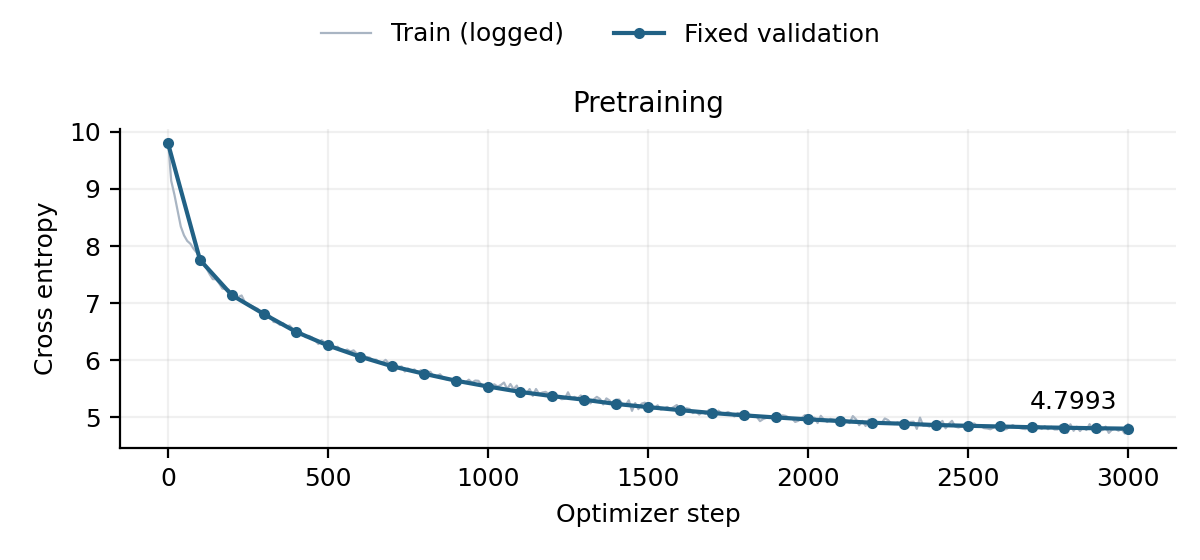
\includegraphics[width=0.86\linewidth]{generated/pretrain_curve.png}

\caption{预训练损失曲线}\label{fig:pretrain}

\end{figure}

固定使用“人工智能技术的发展”“今天上午，学校举办”“随着城市公共交通的发展”三个续写提示。随机种子为42，温度为0.8，top-k为40，最多生成64个新token。第一个提示的随机初始化输出取前80个字符，预训练后输出保留该上限内的完整片段。

\begin{quote}

\begin{minipage}{\linewidth}\small

\textbf{提示}\quad 人工智能技术的发展\par

\textbf{随机初始化}\quad 动摇部件自由贸易场地颂笼罩河流成员国来越来越短暂要在手机闸动机引领役赞同农村─也就是启发耕肇尔特法的启发vel记载变得更被查題样总部设血压尼亚 纽约 民主党警力\par

\textbf{预训练后}\quad :人工智能是人类人类最坏的。人类在人类基因上出现非常明显,其基因是人类进化,人类才有可能灭绝。但人类人类进化了人类。人类认为,人类进化和人类人类的进化成了人类进化的一种新模式。 人类进化论者认为,人类进化学的本质\par

\end{minipage}

\end{quote}

随机初始化输出主要是词语拼接，预训练后开始形成句子结构，但仍反复出现“人类”“进化”等词语。模型对句式和常见词组的学习与验证损失下降相符，连续重复仍反映出语义组织的不足。

\begin{quote}

\begin{minipage}{\linewidth}\small

\textbf{提示}\quad 今天上午，学校举办\par

\textbf{预训练后}\quad 了纪念仪式 这次纪念仪式是出席仪式上。 悼念仪式是今年六月。 曼德拉生前出席,今年5月首次出席曼德拉纪念仪式。 曼德拉与曼德拉同世隔绝, 曼德拉在南非去世4年4月,曼德拉曾成为首届南非总统。 曼德拉今年5月\par

\end{minipage}

\end{quote}

输出从学校活动转向曼德拉纪念仪式，并混合了不同时间表达。新闻语料中的常见实体与事件已经进入生成分布，但模型对提示主题和时间关系的约束仍较弱。本次验证损失由固定窗口估计，生成样例进一步展示了其内容组织能力的边界。


\FloatBarrier
\section{模型微调与任务效果}
\subsection{监督数据与标签构造}
监督任务为根据中文新闻生成标题。初始方案使用清洗后的 text 字段作为新闻输入，title 字段作为目标。训练和生成共用提示格式与新闻截断方式，划分沿用预训练阶段。按第一章的监督目标，提示词末尾位置预测第一个标题 token，最后一个标题 token 预测 EOS，具体关系见表\ref{tab:labels}。

\begin{table}[H]
\centering\small
\caption{微调标签构造}\label{tab:labels}
\begin{tabularx}{\linewidth}{Y l l}
\toprule 输入位置 & 下一 token 标签 & 计入损失 \\ \midrule
提示词内部 & $-100$ & 否 \\
提示词末尾 & 首个标题 token $y_1$ & 是 \\
标题 token $y_j$，$j<m$ & $y_{j+1}$ & 是 \\
最后一个标题 token $y_m$ & EOS & 是 \\
EOS 及其后的填充位置 & $-100$ & 否 \\
\bottomrule
\end{tabularx}
\end{table}

输入使用固定格式。
\begin{quote}\small
请根据以下新闻正文生成一个简洁、准确的中文标题。\\
正文：\textit{新闻内容}\\
标题：\textit{目标标题}
\end{quote}
512-token 上下文中，前缀占 23 token、后缀占 5 token、BOS 占 1 token，标题预留 64 token，因此可见新闻预算为
\begin{equation}
 512-23-5-1-64=419\ \text{token}.
\end{equation}
超出预算的新闻取前缀，右侧填充不参与监督损失。



\subsection{微调策略与训练过程}
比较仅预训练、预训练后微调、随机初始化微调，以及同一可见正文首句前 32 字符的抽取基线。两组微调使用相同模型、词表和采样种子，各训练 1500 步。微批量为 4，累积 8 次，有效批量为 32。最大学习率为 $5\times10^{-5}$，预热 50 步，权重衰减为 0.01。预训练组加载第三章所选检查点，随机初始化组从随机权重开始。

采用全参数微调，各层参与更新，以较小学习率适配新闻到标题的条件关系。1500 步共进行 $1500\times32=48000$ 次有放回样本抽取，累计监督标题及 EOS 共 563358 个 token。监督文本量远少于预训练，随机初始化组需要在这些目标上同时学习语言表示和标题任务。

加载预训练权重后，重新建立 AdamW 优化器并预热学习率。数据经过提示拼接、标签移位和右侧填充后组成批次，损失按有效标题 token 数归一化，再反向传播与更新。

微调每 100 步在固定的 20 个验证批次上估计目标损失，并选择损失最低的检查点。生成评测使用固定的 200 条验证新闻和 500 条测试新闻，各方法使用相同文档。初始评测采用贪心解码，生成上限为 64 个新 token，遇到 EOS 结束。

训练损失在真实标题前缀下计算，生成评测则只输入新闻与提示，让模型使用自己的输出继续生成。后者能够观察重复、偏题和错误信息累积，因而同时保留损失曲线、ROUGE 与逐条输出作为分析依据。

\subsection{初始微调结果与对照}
表\ref{tab:initial}给出同一500条测试新闻上的标题生成结果。预训练后微调的ROUGE-L为28.77，随机初始化微调为9.43，前者高出19.34个分值点。与同输入抽取基线相比，预训练后微调高出5.85个分值点。

\begin{table}[H]
\centering\small
\caption{标题生成对照结果}\label{tab:initial}
\begin{tabularx}{\linewidth}{Y r r r}
\toprule 方法 & ROUGE-1 & ROUGE-2 & ROUGE-L \\ \midrule
首句前32字符 & 26.28 & 14.98 & 22.92 \\
仅预训练 & 2.89 & 1.25 & 2.77 \\
随机初始化微调 & 9.56 & 3.71 & 9.43 \\
预训练后微调 & 30.81 & 17.99 & 28.77 \\
\bottomrule
\end{tabularx}
\end{table}

图\ref{fig:sft}比较两组微调损失，两个子图分别设置纵轴范围。

\begin{figure}[H]

\centering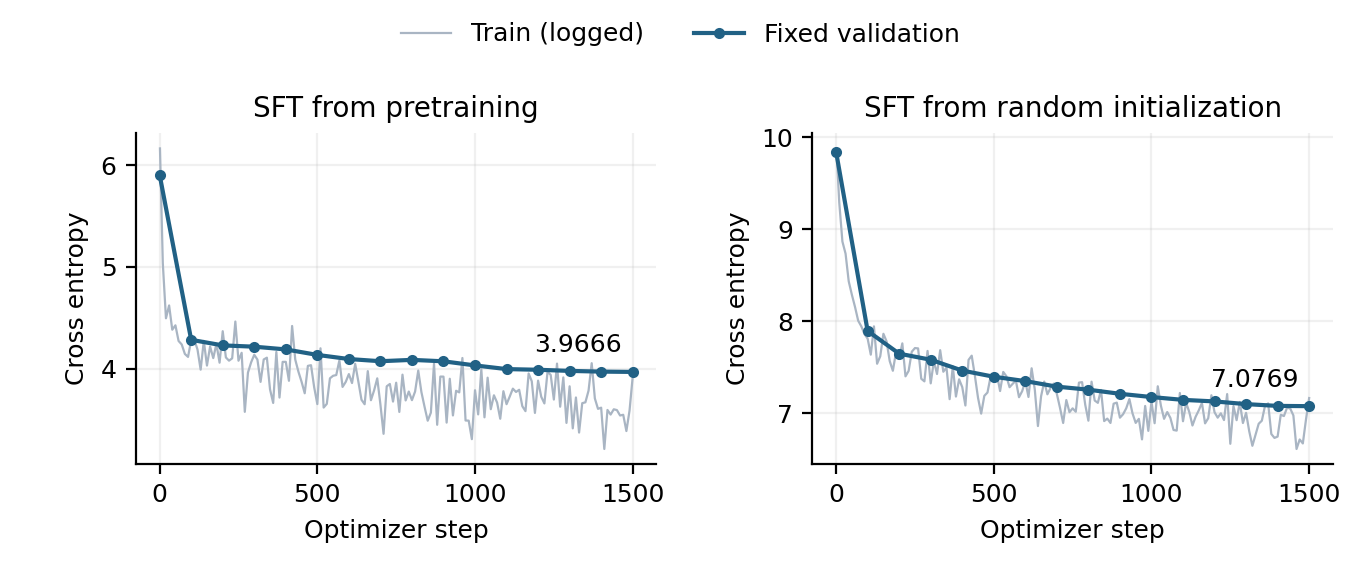
\includegraphics[width=\linewidth]{generated/sft_comparison.png}

\caption{标题微调损失曲线}\label{fig:sft}

\end{figure}

两组最佳验证交叉熵分别为3.9666和7.0769，均出现在第1500步。仅预训练模型的标题得分较低，监督微调有助于学习标题格式和信息选择。预训练组还使用了额外预训练计算，随机初始化组沿用同一微调配置，上述差异反映当前设置下初始化与训练方案的共同影响。

在相同的标题监督范围下，两组固定验证困惑度分别为52.81和1184.25。预训练组更容易利用已有语言表示拟合标题目标。只有预训练时，模型尚未充分适配“读正文、生成标题”的任务格式，因此损失与生成评测共同支持预训练和任务监督分别发挥作用的解释。


\subsection{新闻输入与解码的改进实验}
\subsubsection{信息补全与重复约束}
复查原始新闻发现，部分标题所需事实位于 summary 字段中。该字段有时保留了 text 缺少的导语内容，因此将原始导语放在正文之前，再截取可见输入。模型获得的新闻信息随之发生变化。

对生成重复，比较重复惩罚与禁止重复 token 三元组。重复惩罚只作用于已生成标题中出现过的 token，系数为 $r=1.1$，对应 logit 调整为
\begin{equation}
 z'_v=\begin{cases}z_v/r,&z_v\ge0,\\r z_v,&z_v<0.\end{cases}
\end{equation}
原输入中的实体可以正常复制，解码时取调整后 logit 的最大值。

\subsubsection{分组比较与验证选择}
设置原权重接收正文、原权重接收导语加正文、重新微调后接收导语加正文三组。新增微调从同一个预训练检查点开始，网络、词表、文档顺序、学习率和 1500 步预算与初始微调一致。两种输入都使用 419-token 新闻预算。

每组在相同的 200 条验证新闻上比较贪心解码、重复惩罚 1.1 和禁止重复 token 三元组。按验证 ROUGE-L 选择设置，相同时比较重复提示数，再按声明顺序选择。选定解码后，在相同的 500 条测试新闻上评估。初始测试结果已经用于前期诊断，本轮比较属于在已有测试子集上的后续分析。

\subsubsection{改进结果}
三组验证结果见表\ref{tab:validation}，均由重复惩罚1.1获得最高ROUGE-L，因此采用该设置进入测试。

\begin{table}[H]
\centering\small
\caption{解码方法比较}\label{tab:validation}
\begin{tabularx}{\linewidth}{Y r r r}
\toprule 模型与新闻输入 & 贪心 & 惩罚1.1 & 禁重复3-gram \\ \midrule
原微调权重，正文 & 27.88 & 28.03 & 27.96 \\
原微调权重，导语加正文 & 29.84 & 30.57 & 30.04 \\
重新微调权重，导语加正文 & 35.21 & 35.63 & 35.14 \\
\bottomrule
\end{tabularx}
\end{table}

\begin{table}[H]
\centering\small
\caption{输入与微调改进结果}\label{tab:refinement}
\begin{tabularx}{\linewidth}{Y l r r r}
\toprule 模型 & 新闻输入 & ROUGE-1 & ROUGE-2 & ROUGE-L \\ \midrule
原微调权重 & 正文 & 31.72 & 18.64 & 29.37 \\
原微调权重 & 导语加正文 & 34.47 & 20.70 & 31.80 \\
重新微调权重 & 导语加正文 & 38.77 & 24.44 & 35.86 \\
首句抽取 & 导语加正文 & 33.34 & 20.24 & 29.41 \\
\bottomrule
\end{tabularx}
\end{table}

表\ref{tab:refinement}中，原权重使用正文并调整解码后，ROUGE-L为29.37，比初始贪心结果高0.60个分值点。加入导语后达到31.80，再提高2.43个分值点。在相同输入和解码下，重新微调达到35.86，相对原权重提高4.06个分值点，相对同输入抽取基线提高6.45个分值点。

总分变化包含解码、输入信息和重新微调三项因素，各项增量依赖当前条件。新增微调的最佳验证交叉熵为3.6074，训练迭代用时9.1分钟。

\begin{figure}[H]

\centering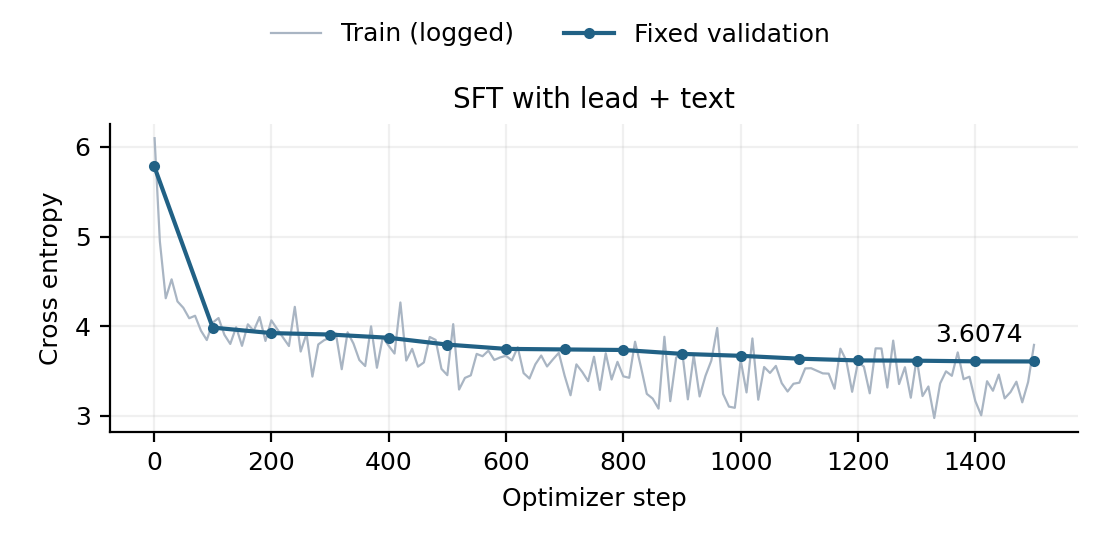
\includegraphics[width=0.82\linewidth]{generated/refinement_curve.png}

\caption{改进微调损失曲线}\label{fig:refinement}

\end{figure}


\subsection{标题生成样例与错误分析}
表\ref{tab:examples}按文档ID顺序展示固定测试子集的前四条。初始方案输入正文，最终方案输入导语加正文。

\begin{table}[H]
\centering\small
\caption{标题生成样例}\label{tab:examples}
\begin{tabularx}{\linewidth}{Y Y Y}
\toprule 参考标题 & 初始方案 & 最终方案 \\ \midrule
动物特工: 俄罗斯白鲸和其他那些飞禽走兽 & “间谍”的间谍:\ReportAnimalPronoun{}们为什么会“间谍” & 间谍:\ReportAnimalPronoun{}们不服的“间谍” \\
香港学生罢课 台湾学生声援 朝野关注 & 台湾学生声援香港占中 & 台湾太阳花:陈为廷称香港罢课是“民主” \\
媒体报道揭示上海自由贸易区管理安排 & 北京将上海自贸区列入“国际金融中心” & 上海将设立自贸区 \\
北京两会期间周永康再次受到媒体关注 & 周滨为周永康之子周滨 & 周滨为周永康之子 \\
\bottomrule
\end{tabularx}
\end{table}

样例中有些重复减少，上海自贸区新闻的输出也更贴近事件主题，但动物特工样例仍存在语义不清的问题。为进一步观察数字和事件关系，从按文档ID排序的前8条验证样例中取以下两例。

\begin{quote}\small

\textbf{输入片段}\quad 有报道说,巴黎地区警方前夜扣押12名涉嫌支持上周当地恐怖袭击的嫌疑犯。\par

\textbf{生成标题}\quad 巴黎袭击案:警方前夜逮捕7名嫌疑人\par

\end{quote}

导语明确给出12名嫌疑犯，输出仍写成7名，具体人数被错误生成。

\begin{quote}\small

\textbf{输入片段}\quad 海协会会长陈云林在完成六次陈江会后周三(12月22日)中午离开台湾,他此行在台湾如同过往到访一样,受到不断的抗议与甚高规格的维安保护。\par

\textbf{生成标题}\quad 台湾来鸿:六四后两岸和平大趋势\par

\end{quote}

导语描述完成六次陈江会后离台，输出却出现“六四后”，改变了事件含义。

初始贪心输出中，四字符片段至少重复三次的提示有17条，最终方案降至2条。最终输出中还有18条数字片段未直接出现在完整输入中。这些规则用于定位待复核样本，事实判断还需检查上下文与表达转换。上述案例表明，输入补全和重复约束之后，数字与事件关系仍可能出错。


\FloatBarrier
\section{成果总结与体会}
本次从随机权重搭建了约 5000 万参数的中文 GPT，完成中文新闻预训练和标题生成微调。预训练验证交叉熵由 9.7996 降至 4.7993，初始微调的 ROUGE-L 为 28.77，高于随机初始化微调的 9.43。加入导语并重新微调后，ROUGE-L 达到 35.86，同输入抽取基线为 29.41。模型已经能够生成部分与新闻主题相符的标题，数字和事件关系仍有错误。

手写模型的过程使我对 Transformer 中的张量运算有了更具体的理解。实现多头注意力时，需要将 $(B,T,d)$ 的表示拆成 $(B,h,T,d/h)$，分别计算各头的注意力，再恢复原来的形状。逐步核对投影、转置、拼接与输出维度后，我能够把公式中的每一步与前向传播对应起来。对照手写矩阵版本与 SDPA 的输出和梯度，也让我理解了高层计算接口所完成的具体运算。

训练目标的实现同样加深了我的理解。预训练中，输入与标签错开一个位置，当前位置根据已有前缀预测下一个 token。微调时，还需要把提示和填充对应的标签设为 $-100$，只在标题与 EOS 上计算损失。检查“提示末尾预测第一个标题 token”这一对应关系，让我认识到张量形状正确之后，还需要核对每个位置实际学习的目标。因果遮罩测试则帮助我验证模型是否读取了未来信息。

在训练程序中，我进一步理解了梯度累积、优化器更新和断点恢复之间的关系。微调样本的标题长度不同，因此需要按有效监督 token 总数计算平均损失。检查点还要保存优化器和随机数状态，才能接续原来的抽样与更新。通过小型合成任务和中断恢复检查，我学会了先验证基本计算与训练流程，再运行正式实验。

结果分析使我体会到，模型效果还取决于输入信息是否完整。检查新闻正文与生成样例后，发现导语中包含部分标题所需事实，补充导语后指标进一步提高。对照具体输出仍能看到人数错误和事件含义变化，因此我在评价时同时查看损失、ROUGE 和生成内容。今后还需要用新的评测样本和多随机种子实验检验结果，并进一步检查实体与数字的一致性。

项目的模型、数据处理、训练、评测与推理代码已整理开源，仓库中提供环境配置和复现步骤，地址为 \url{https://github.com/Lyrah12/mini-gpt-from-scratch}。

\begin{thebibliography}{9}
\bibitem{transformer} Vaswani A, et al. Attention Is All You Need. 2017.\\
\url{https://arxiv.org/abs/1706.03762}
\bibitem{fromscratch} Raschka S. LLMs from Scratch.\\
\url{https://github.com/rasbt/LLMs-from-scratch}
\bibitem{xlsum} Hasan T, et al. XL-Sum 中文新闻数据集.\\
\url{https://huggingface.co/datasets/csebuetnlp/xlsum}
\end{thebibliography}

\end{document}
